% leetcuda_cover_bench.tex — LeetCUDA 封面 + bench 表格 横向合并图（手绘风, 两图各带手绘边框）
% 合并自: kernels/interview/book/figures/misc/cover-tikz.tex (封面, A4 竖版 21x29.7cm)
%         docs/leetcuda_bench_table.tex (bench 数据表)
% 布局: 封面在左, 表格在右且垂直居中对齐封面; 自包含单文件, 不依赖被合并的两个 tex
% 构建: xelatex leetcuda_cover_bench.tex  (standalone 单页 PDF)
\documentclass[tikz,border=12pt]{standalone}
\usetikzlibrary{arrows.meta,calc,decorations.pathmorphing}
\usepackage{xeCJK}
\usepackage{amsmath}
\setmainfont{Humor Sans}
\setsansfont{Humor Sans}
\setmonofont{Comic Neue}
\setCJKmainfont{LXGW WenKai}
\setCJKsansfont{LXGW WenKai}
\renewcommand{\familydefault}{\sfdefault}

\tikzset{
  sketch/.style={decorate, decoration={random steps, segment length=2.5mm, amplitude=0.3mm}},
  sketchfine/.style={decorate, decoration={random steps, segment length=8mm, amplitude=0.15mm}}}

% 封面配色 (colfax quotient ramp, jewel-tone 降饱和)
\definecolor{coverBg}{RGB}{248,249,251}
\definecolor{coverInk}{RGB}{31,35,40}
\definecolor{coverMuted}{RGB}{118,126,138}
\definecolor{accentBlue}{RGB}{33,113,181}
\definecolor{colorx1}{RGB}{213,84,76}
\definecolor{colorx2}{RGB}{232,163,61}
\definecolor{colorx3}{RGB}{155,191,90}
\definecolor{colorx4}{RGB}{76,182,149}
\definecolor{colorx5}{RGB}{69,168,200}
\definecolor{colorx6}{RGB}{62,124,192}
\definecolor{colorx7}{RGB}{126,99,184}
\definecolor{colorx8}{RGB}{194,88,158}

% 表格配色
\definecolor{colBlue}{HTML}{2F6FB5}
\definecolor{colRed}{HTML}{C93A31}
\definecolor{colOrange}{HTML}{C87A0A}
\definecolor{colGreen}{HTML}{227A32}
\definecolor{colPurple}{HTML}{7A4FA3}
\definecolor{colTeal}{HTML}{127F87}
\definecolor{colAccent}{HTML}{3B3A8F}
\definecolor{colGray}{HTML}{5A5A5A}

% 表格字体
\def\subfont{\fontsize{11pt}{13pt}\selectfont}
\def\capfont{\fontsize{7pt}{8.8pt}\selectfont}
\def\hdffont{\fontsize{8pt}{10pt}\selectfont}
\def\grpfont{\fontsize{8pt}{10pt}\selectfont}
\def\rowfont{\fontsize{8.5pt}{10.5pt}\selectfont}

\pgfmathsetseed{7}

% wiggly rule: [style] x0 / x1 / y
\newcommand{\wrule}[4][line width=0.9pt]{%
  \draw[#1, decorate, decoration={random steps, segment length=7pt, amplitude=0.55pt}]
    (#2,#4) -- (#3,#4);}

% TFLOPS bars, left table scaled to 250, right tables to 500 / 210
% (right top holds both HGEMM and FP8, so it needs one axis wide enough for ~490 T)
\newcommand{\lbar}[3]{%
  \pgfmathsetmacro{\bw}{#2/250*1.8}%
  \fill[#3] (5.95,{#1-0.075}) rectangle ++(\bw cm,0.15);}
\newcommand{\rbarA}[3]{%
  \pgfmathsetmacro{\bw}{#2/500*1.65}%
  \fill[#3] (14.80,{#1-0.075}) rectangle ++(\bw cm,0.15);}
\newcommand{\rbarB}[3]{%
  \pgfmathsetmacro{\bw}{#2/210*1.65}%
  \fill[#3] (14.80,{#1-0.075}) rectangle ++(\bw cm,0.15);}

% data row: y / config / TFLOPS / speedup / color
\newcommand{\lrow}[5]{%
  \node[anchor=west, font=\rowfont, inner sep=0pt] at (0,#1) {#2};%
  \node[anchor=east, font=\rowfont, inner sep=0pt] at (4.20,#1) {#3};%
  \node[anchor=east, font=\rowfont, inner sep=0pt, text=#5] at (5.60,#1) {#4};%
  \lbar{#1}{#3}{#5}}

\newcommand{\rrowA}[5]{%
  \node[anchor=west, font=\rowfont, inner sep=0pt] at (8.60,#1) {#2};%
  \node[anchor=east, font=\rowfont, inner sep=0pt] at (13.10,#1) {#3};%
  \node[anchor=east, font=\rowfont, inner sep=0pt, text=#5] at (14.50,#1) {#4};%
  \rbarA{#1}{#3}{#5}}

\newcommand{\rrowB}[5]{%
  \node[anchor=west, font=\rowfont, inner sep=0pt] at (8.60,#1) {#2};%
  \node[anchor=east, font=\rowfont, inner sep=0pt] at (13.10,#1) {#3};%
  \node[anchor=east, font=\rowfont, inner sep=0pt, text=#5] at (14.50,#1) {#4};%
  \rbarB{#1}{#3}{#5}}

% group heading: separated? / y / color / text
\newcommand{\lgrp}[4]{%
  \ifnum#1=1 \wrule[draw=black!20, line width=0.5pt]{0}{7.75}{#2+0.30}\fi
  \fill[#3] (0,{#2-0.075}) rectangle ++(0.17,0.17);%
  \node[anchor=west, font=\grpfont, inner sep=0pt, text=#3] at (0.30,#2) {#4};}
\newcommand{\rgrp}[4]{%
  \ifnum#1=1 \wrule[draw=black!20, line width=0.5pt]{8.60}{17.55}{#2+0.30}\fi
  \fill[#3] (8.60,{#2-0.075}) rectangle ++(0.17,0.17);%
  \node[anchor=west, font=\grpfont, inner sep=0pt, text=#3] at (8.90,#2) {#4};}

\begin{document}
\begin{tikzpicture}

% ===================== LEFT: COVER (等比缩放至与 bench 节点等高) =====================
% \covscale = (benchH(393.91068pt) - 6pt inner sep) / 29.7cm 封面 = 0.460763
% (node scale 不缩放 inner sep, 故先扣除)
\node[inner sep=3pt, scale=0.460763, transform shape] (cover) at (0,0)
  {\begin{tikzpicture}
% ===== A4 背景 (cm), 极淡冷灰渐变 =====
\shade[top color=coverBg, bottom color=coverBg!94!accentBlue] (0,0) rectangle (21,29.7);

% ===== 背景装饰: 散落 size:stride 元组纹理 (浅灰) =====
\node[rotate=12, anchor=center, text=coverMuted!35, font=\ttfamily\footnotesize] at (2.3,24.3) {(4,8):(8,1)};
\node[rotate=-12, anchor=center, text=coverMuted!35, font=\ttfamily\footnotesize] at (18.7,24.3) {(128,128):(1,128)};
\node[rotate=7, anchor=center, text=coverMuted!30, font=\ttfamily\footnotesize] at (2.3,17.6) {((2,2),(2,2))};
\node[rotate=-7, anchor=center, text=coverMuted!30, font=\ttfamily\footnotesize] at (18.7,17.6) {(3):(1)};
\node[rotate=-6, anchor=center, text=coverMuted!28, font=\ttfamily\footnotesize] at (2.3,7.0) {(16,8):(8,1)};
\node[rotate=6, anchor=center, text=coverMuted!28, font=\ttfamily\footnotesize] at (18.7,7.0) {(8,16):(1,8)};

% ===== 顶部小标签 =====
\node[text=coverMuted, font=\ttfamily\bfseries\small] at (10.5,26.9)
  {CUTE\; LAYOUT $\cdot$ TENSOR\; CORE $\cdot$ FLASH\; ATTENTION};

% ===== 标题块 =====
\node[text=coverInk, font=\fontsize{44}{48}\selectfont\bfseries] at (10.5,23.9) {LeetCUDA};
\node[text=coverInk, font=\fontsize{25}{30}\selectfont\bfseries] at (10.5,21.3)
  {\CJKfamily{zhsans}\sffamily CUDA Kernel 优化之路};
\node[text=coverMuted, font=\fontsize{13}{16}\selectfont] at (10.5,19.5)
  {从编程模型到 CuTe 与 FlashAttention};

% colorx 八段细色条 (与网格 8 hue 呼应, 极细低调)
\foreach \i in {0,...,7} {%
  \fill[colorx\number\numexpr\i+1\relax!85] (3.3+\i*1.8,18.55) rectangle +(1.8,0.06);}

% ===== 主视觉: CuTe layout 网格 (8x16) =====
% L = (8,16):(1,8); hue = 2 列 tile 组, intensity = 行渐变 (quotient ramp)
\begin{scope}[shift={(3.75,15.5)}, x={(0cm,-0.9cm)}, y={(0.9cm,0cm)},
  every node/.style={minimum size=0.9cm, outer sep=0pt, text=coverInk!65,
    font=\fontsize{7.5}{8.5}\selectfont}]
  \node[fill=colorx1!8] at (0,0) {0};
\node[fill=colorx1!8] at (0,1) {8};
\node[fill=colorx2!8] at (0,2) {16};
\node[fill=colorx2!8] at (0,3) {24};
\node[fill=colorx3!8] at (0,4) {32};
\node[fill=colorx3!8] at (0,5) {40};
\node[fill=colorx4!8] at (0,6) {48};
\node[fill=colorx4!8] at (0,7) {56};
\node[fill=colorx5!8] at (0,8) {64};
\node[fill=colorx5!8] at (0,9) {72};
\node[fill=colorx6!8] at (0,10) {80};
\node[fill=colorx6!8] at (0,11) {88};
\node[fill=colorx7!8] at (0,12) {96};
\node[fill=colorx7!8] at (0,13) {104};
\node[fill=colorx8!8] at (0,14) {112};
\node[fill=colorx8!8] at (0,15) {120};
\node[fill=colorx1!16] at (1,0) {1};
\node[fill=colorx1!16] at (1,1) {9};
\node[fill=colorx2!16] at (1,2) {17};
\node[fill=colorx2!16] at (1,3) {25};
\node[fill=colorx3!16] at (1,4) {33};
\node[fill=colorx3!16] at (1,5) {41};
\node[fill=colorx4!16] at (1,6) {49};
\node[fill=colorx4!16] at (1,7) {57};
\node[fill=colorx5!16] at (1,8) {65};
\node[fill=colorx5!16] at (1,9) {73};
\node[fill=colorx6!16] at (1,10) {81};
\node[fill=colorx6!16] at (1,11) {89};
\node[fill=colorx7!16] at (1,12) {97};
\node[fill=colorx7!16] at (1,13) {105};
\node[fill=colorx8!16] at (1,14) {113};
\node[fill=colorx8!16] at (1,15) {121};
\node[fill=colorx1!24] at (2,0) {2};
\node[fill=colorx1!24] at (2,1) {10};
\node[fill=colorx2!24] at (2,2) {18};
\node[fill=colorx2!24] at (2,3) {26};
\node[fill=colorx3!24] at (2,4) {34};
\node[fill=colorx3!24] at (2,5) {42};
\node[fill=colorx4!24] at (2,6) {50};
\node[fill=colorx4!24] at (2,7) {58};
\node[fill=colorx5!24] at (2,8) {66};
\node[fill=colorx5!24] at (2,9) {74};
\node[fill=colorx6!24] at (2,10) {82};
\node[fill=colorx6!24] at (2,11) {90};
\node[fill=colorx7!24] at (2,12) {98};
\node[fill=colorx7!24] at (2,13) {106};
\node[fill=colorx8!24] at (2,14) {114};
\node[fill=colorx8!24] at (2,15) {122};
\node[fill=colorx1!32] at (3,0) {3};
\node[fill=colorx1!32] at (3,1) {11};
\node[fill=colorx2!32] at (3,2) {19};
\node[fill=colorx2!32] at (3,3) {27};
\node[fill=colorx3!32] at (3,4) {35};
\node[fill=colorx3!32] at (3,5) {43};
\node[fill=colorx4!32] at (3,6) {51};
\node[fill=colorx4!32] at (3,7) {59};
\node[fill=colorx5!32] at (3,8) {67};
\node[fill=colorx5!32] at (3,9) {75};
\node[fill=colorx6!32] at (3,10) {83};
\node[fill=colorx6!32] at (3,11) {91};
\node[fill=colorx7!32] at (3,12) {99};
\node[fill=colorx7!32] at (3,13) {107};
\node[fill=colorx8!32] at (3,14) {115};
\node[fill=colorx8!32] at (3,15) {123};
\node[fill=colorx1!40] at (4,0) {4};
\node[fill=colorx1!40] at (4,1) {12};
\node[fill=colorx2!40] at (4,2) {20};
\node[fill=colorx2!40] at (4,3) {28};
\node[fill=colorx3!40] at (4,4) {36};
\node[fill=colorx3!40] at (4,5) {44};
\node[fill=colorx4!40] at (4,6) {52};
\node[fill=colorx4!40] at (4,7) {60};
\node[fill=colorx5!40] at (4,8) {68};
\node[fill=colorx5!40] at (4,9) {76};
\node[fill=colorx6!40] at (4,10) {84};
\node[fill=colorx6!40] at (4,11) {92};
\node[fill=colorx7!40] at (4,12) {100};
\node[fill=colorx7!40] at (4,13) {108};
\node[fill=colorx8!40] at (4,14) {116};
\node[fill=colorx8!40] at (4,15) {124};
\node[fill=colorx1!48] at (5,0) {5};
\node[fill=colorx1!48] at (5,1) {13};
\node[fill=colorx2!48] at (5,2) {21};
\node[fill=colorx2!48] at (5,3) {29};
\node[fill=colorx3!48] at (5,4) {37};
\node[fill=colorx3!48] at (5,5) {45};
\node[fill=colorx4!48] at (5,6) {53};
\node[fill=colorx4!48] at (5,7) {61};
\node[fill=colorx5!48] at (5,8) {69};
\node[fill=colorx5!48] at (5,9) {77};
\node[fill=colorx6!48] at (5,10) {85};
\node[fill=colorx6!48] at (5,11) {93};
\node[fill=colorx7!48] at (5,12) {101};
\node[fill=colorx7!48] at (5,13) {109};
\node[fill=colorx8!48] at (5,14) {117};
\node[fill=colorx8!48] at (5,15) {125};
\node[fill=colorx1!56] at (6,0) {6};
\node[fill=colorx1!56] at (6,1) {14};
\node[fill=colorx2!56] at (6,2) {22};
\node[fill=colorx2!56] at (6,3) {30};
\node[fill=colorx3!56] at (6,4) {38};
\node[fill=colorx3!56] at (6,5) {46};
\node[fill=colorx4!56] at (6,6) {54};
\node[fill=colorx4!56] at (6,7) {62};
\node[fill=colorx5!56] at (6,8) {70};
\node[fill=colorx5!56] at (6,9) {78};
\node[fill=colorx6!56] at (6,10) {86};
\node[fill=colorx6!56] at (6,11) {94};
\node[fill=colorx7!56] at (6,12) {102};
\node[fill=colorx7!56] at (6,13) {110};
\node[fill=colorx8!56] at (6,14) {118};
\node[fill=colorx8!56] at (6,15) {126};
\node[fill=colorx1!64] at (7,0) {7};
\node[fill=colorx1!64] at (7,1) {15};
\node[fill=colorx2!64] at (7,2) {23};
\node[fill=colorx2!64] at (7,3) {31};
\node[fill=colorx3!64] at (7,4) {39};
\node[fill=colorx3!64] at (7,5) {47};
\node[fill=colorx4!64] at (7,6) {55};
\node[fill=colorx4!64] at (7,7) {63};
\node[fill=colorx5!64] at (7,8) {71};
\node[fill=colorx5!64] at (7,9) {79};
\node[fill=colorx6!64] at (7,10) {87};
\node[fill=colorx6!64] at (7,11) {95};
\node[fill=colorx7!64] at (7,12) {103};
\node[fill=colorx7!64] at (7,13) {111};
\node[fill=colorx8!64] at (7,14) {119};
\node[fill=colorx8!64] at (7,15) {127};
  % 手绘风: 只画内部网格线; 外边界由墨线框覆盖 (避免白线与墨框双层错位)
  \foreach \a in {0.5,1.5,...,6.5} \draw[white, line width=0.7pt, sketchfine] (\a,-0.5) -- (\a,15.5);
  \foreach \b in {0.5,1.5,...,14.5} \draw[white, line width=0.7pt, sketchfine] (-0.5,\b) -- (7.5,\b);
  \draw[coverInk!35, line width=0.7pt, sketch] (-0.5,-0.5) rectangle (7.5,15.5);
\end{scope}

% 高亮 tile B = (2,2):(1,8) (右上角 2x2 tile, accent 粗框; scope 内 i0 行 0-1, i1 列 14-15)
\draw[accentBlue, line width=1.5pt, rounded corners=1.5pt, sketch,
  shift={(3.75,15.5)}, x={(0cm,-0.9cm)}, y={(0.9cm,0cm)}]
  (-0.5,13.5) rectangle (1.5,15.5);
\node[anchor=south, text=accentBlue, font=\ttfamily\bfseries\footnotesize]
  at (16.8,16.85) {B = (2,2):(1,8)};
\draw[-{Stealth[length=1.8mm]}, accentBlue, line width=0.8pt, sketch] (16.8,16.7) -- (16.8,16.0);

% layout 方程 (网格正下方, 居中)
\node[text=coverInk, font=\fontsize{13}{16}\selectfont] at (10.5,7.7)
  {L = (8,16):(1,8)};
% mode 标注: mode0 (stride 1) 向下, mode1 (stride 8) 向右
\node[rotate=90, anchor=center, text=coverMuted, font=\ttfamily\footnotesize] at (2.95,12.35) {mode\,0\,:\,(1)\;$\downarrow$};
\node[text=coverMuted, font=\ttfamily\footnotesize] at (10.5,16.35) {$\rightarrow$\;mode\,1\,:\,(8)};

% TiledMMA 代码块 (单行; 卡片与网格同宽对齐, 编辑器窗口风格)
\draw[fill=white!30!coverBg!95!accentBlue, draw=coverInk!35, line width=0.6pt, rounded corners=2.5pt, sketch]
  (3.3,6.0) rectangle (17.7,7.0);
\foreach \i/\c in {0/colorx1,1/colorx2,2/colorx4}
  \fill[\c!80] (3.62+\i*0.2,6.83) circle (0.052);
\node[anchor=center, text=coverMuted, font=\ttfamily\small] at (10.5,6.36)
  {auto tiled\_mma = {\color{accentBlue}make\_tiled\_mma}(SM80\_16x8x16\_F32F16F16F32\_TN\{\}, Layout<Shape<\_2,\_2,\_1>>\{\});};

% ===== 底部声明 (细线框) =====
\node[draw=accentBlue!45, sketch, rounded corners=2pt, inner xsep=10pt, inner ysep=8pt,
  text=coverInk, text width=13.7cm, align=center, font=\small] at (10.5,4.75)
  {\CJKfamily{zhsans}\bfseries 郑重声明\\
   \mdseries\CJKfamily{zhsong} 本书仅用于开源学习与技术交流，\\未经作者本人同意，不得用于任何商业用途。};
\node[text=coverMuted, font=\small] at (10.5,2.85)
  {LeetCUDA Project (Own by DefTruth) $\cdot$ 2026 年 9 月};
  \end{tikzpicture}};

% ===================== RIGHT: BENCH TABLE =====================
\node[inner sep=6pt, anchor=west] (bench) at ($(cover.east)+(0.4cm,0)$)
  {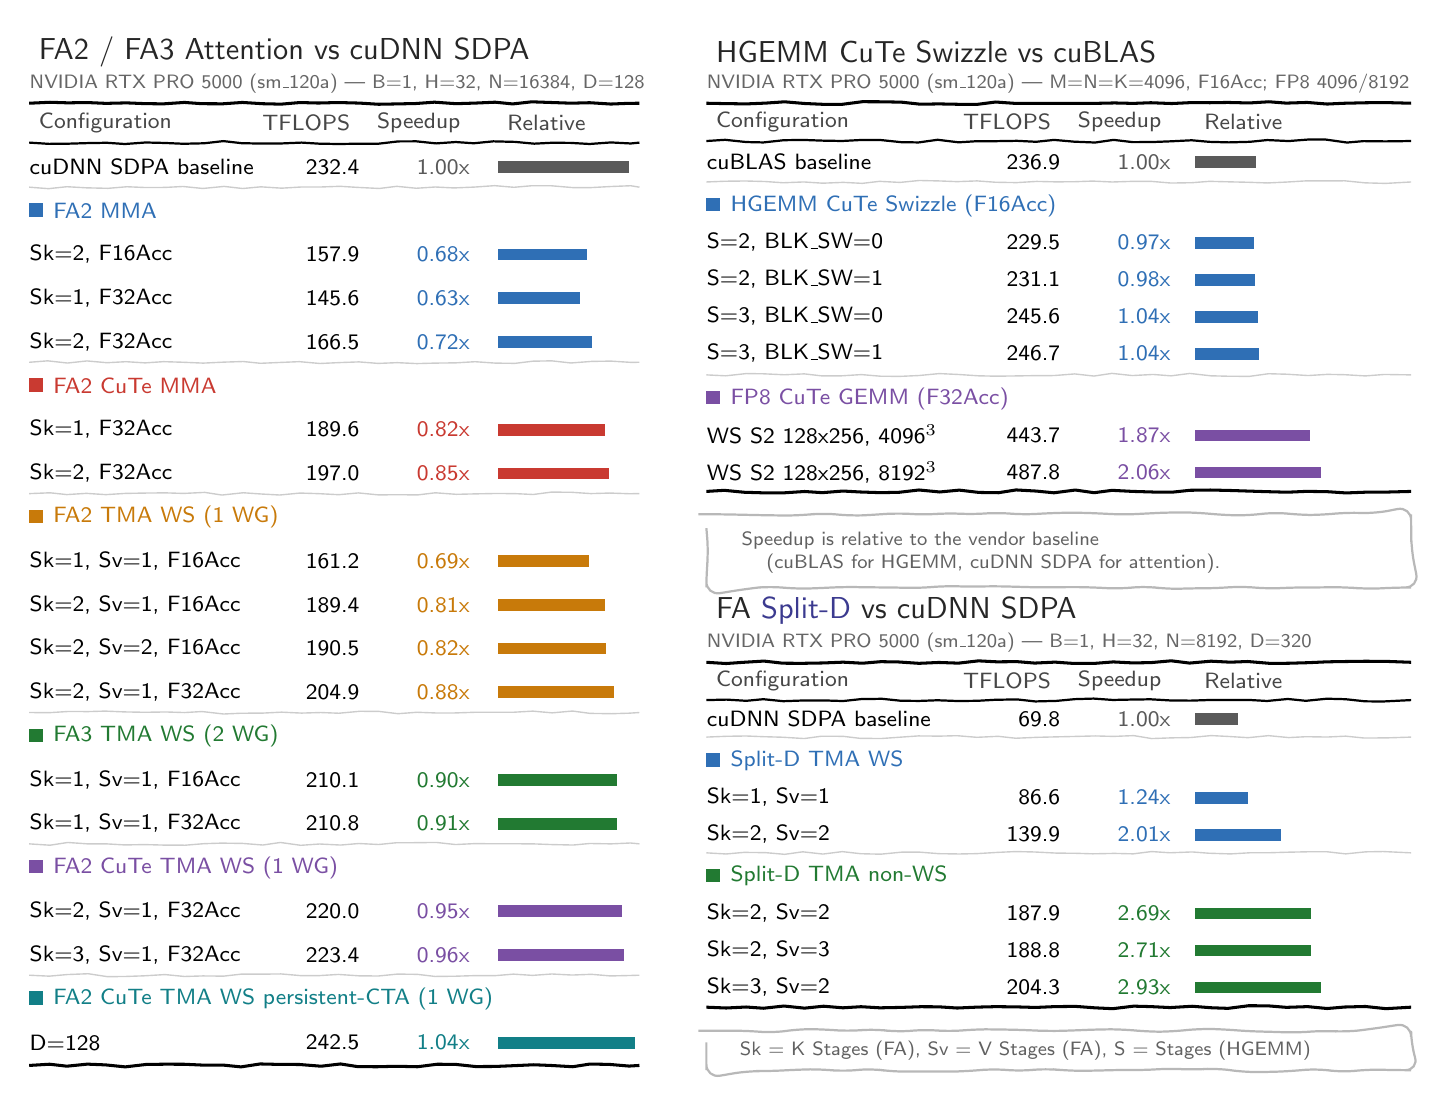
\begin{tikzpicture}
% ===================== LEFT: FA2 / FA3 vs cuDNN SDPA =====================
\node[anchor=west, font=\subfont, text=black!85] at (0,-0.35)
  {FA2 / FA3 Attention vs cuDNN SDPA};
\node[anchor=north west, font=\capfont, text=black!60, align=left, inner sep=0pt] at (0,-0.62)
  {NVIDIA RTX PRO 5000 (sm\_120a) --- B=1, H=32, N=16384, D=128};

\wrule[line width=1.1pt]{0}{7.75}{-1.00}
\node[anchor=west, font=\hdffont, text=black!72] at (0,-1.25) {Configuration};
\node[anchor=east, font=\hdffont, text=black!72] at (4.20,-1.25) {TFLOPS};
\node[anchor=east, font=\hdffont, text=black!72] at (5.60,-1.25) {Speedup};
\node[anchor=west, font=\hdffont, text=black!72] at (5.95,-1.25) {Relative};
\wrule[line width=0.8pt]{0}{7.75}{-1.50}

\lrow{-1.810}{cuDNN SDPA baseline}{232.4}{1.00x}{colGray}

\lgrp{1}{-2.366}{colBlue}{FA2 MMA}
\lrow{-2.922}{Sk=2, F16Acc}{157.9}{0.68x}{colBlue}
\lrow{-3.478}{Sk=1, F32Acc}{145.6}{0.63x}{colBlue}
\lrow{-4.034}{Sk=2, F32Acc}{166.5}{0.72x}{colBlue}

\lgrp{1}{-4.590}{colRed}{FA2 CuTe MMA}
\lrow{-5.146}{Sk=1, F32Acc}{189.6}{0.82x}{colRed}
\lrow{-5.702}{Sk=2, F32Acc}{197.0}{0.85x}{colRed}

\lgrp{1}{-6.258}{colOrange}{FA2 TMA WS (1 WG)}
\lrow{-6.814}{Sk=1, Sv=1, F16Acc}{161.2}{0.69x}{colOrange}
\lrow{-7.370}{Sk=2, Sv=1, F16Acc}{189.4}{0.81x}{colOrange}
\lrow{-7.926}{Sk=2, Sv=2, F16Acc}{190.5}{0.82x}{colOrange}
\lrow{-8.482}{Sk=2, Sv=1, F32Acc}{204.9}{0.88x}{colOrange}

\lgrp{1}{-9.038}{colGreen}{FA3 TMA WS (2 WG)}
\lrow{-9.594}{Sk=1, Sv=1, F16Acc}{210.1}{0.90x}{colGreen}
\lrow{-10.150}{Sk=1, Sv=1, F32Acc}{210.8}{0.91x}{colGreen}

\lgrp{1}{-10.706}{colPurple}{FA2 CuTe TMA WS (1 WG)}
\lrow{-11.262}{Sk=2, Sv=1, F32Acc}{220.0}{0.95x}{colPurple}
\lrow{-11.818}{Sk=3, Sv=1, F32Acc}{223.4}{0.96x}{colPurple}

\lgrp{1}{-12.374}{colTeal}{FA2 CuTe TMA WS persistent-CTA (1 WG)}
\lrow{-12.930}{D=128}{242.5}{1.04x}{colTeal}

\wrule[line width=1.1pt]{0}{7.75}{-13.22}

% ===================== RIGHT TOP: HGEMM / FP8 vs cuBLAS =====================
\node[anchor=west, font=\subfont, text=black!85] at (8.60,-0.35)
  {HGEMM CuTe Swizzle vs cuBLAS};
\node[anchor=north west, font=\capfont, text=black!60, align=left, inner sep=0pt] at (8.60,-0.62)
  {NVIDIA RTX PRO 5000 (sm\_120a) --- M=N=K=4096, F16Acc; FP8 4096/8192};

\wrule[line width=1.1pt]{8.60}{17.55}{-1.00}
\node[anchor=west, font=\hdffont, text=black!72] at (8.60,-1.24) {Configuration};
\node[anchor=east, font=\hdffont, text=black!72] at (13.10,-1.24) {TFLOPS};
\node[anchor=east, font=\hdffont, text=black!72] at (14.50,-1.24) {Speedup};
\node[anchor=west, font=\hdffont, text=black!72] at (14.80,-1.24) {Relative};
\wrule[line width=0.8pt]{8.60}{17.55}{-1.48}

\rrowA{-1.75}{cuBLAS baseline}{236.9}{1.00x}{colGray}

\rgrp{1}{-2.30}{colBlue}{HGEMM CuTe Swizzle (F16Acc)}
\rrowA{-2.77}{S=2, BLK\_SW=0}{229.5}{0.97x}{colBlue}
\rrowA{-3.24}{S=2, BLK\_SW=1}{231.1}{0.98x}{colBlue}
\rrowA{-3.71}{S=3, BLK\_SW=0}{245.6}{1.04x}{colBlue}
\rrowA{-4.18}{S=3, BLK\_SW=1}{246.7}{1.04x}{colBlue}

\rgrp{1}{-4.75}{colPurple}{FP8 CuTe GEMM (F32Acc)}
\rrowA{-5.22}{WS S2 128x256, 4096$^3$}{443.7}{1.87x}{colPurple}
\rrowA{-5.69}{WS S2 128x256, 8192$^3$}{487.8}{2.06x}{colPurple}

\wrule[line width=1.1pt]{8.60}{17.55}{-5.93}

\node[anchor=north west, font=\fontsize{7pt}{8.2pt}\selectfont, text=black!62,
      align=left, inner sep=4pt]
  at (8.90,-6.30) {Speedup is relative to the vendor baseline\\\hspace*{1.2em}(cuBLAS for HGEMM, cuDNN SDPA for attention).};
\draw[draw=black!28, line width=0.8pt, decorate,
      decoration={random steps, segment length=9pt, amplitude=0.8pt}, rounded corners=5pt]
  (8.60,-6.22) rectangle (17.55,-7.15);

% ===================== RIGHT BOTTOM: FA Split-D vs cuDNN SDPA =====================
\node[anchor=west, font=\subfont, text=black!85] at (8.60,-7.45)
  {FA \textcolor{colAccent}{Split-D} vs cuDNN SDPA};
\node[anchor=north west, font=\capfont, text=black!60, align=left, inner sep=0pt] at (8.60,-7.72)
  {NVIDIA RTX PRO 5000 (sm\_120a) --- B=1, H=32, N=8192, D=320};

\wrule[line width=1.1pt]{8.60}{17.55}{-8.10}
\node[anchor=west, font=\hdffont, text=black!72] at (8.60,-8.34) {Configuration};
\node[anchor=east, font=\hdffont, text=black!72] at (13.10,-8.34) {TFLOPS};
\node[anchor=east, font=\hdffont, text=black!72] at (14.50,-8.34) {Speedup};
\node[anchor=west, font=\hdffont, text=black!72] at (14.80,-8.34) {Relative};
\wrule[line width=0.8pt]{8.60}{17.55}{-8.58}

\rrowB{-8.82}{cuDNN SDPA baseline}{69.8}{1.00x}{colGray}

\rgrp{1}{-9.35}{colBlue}{Split-D TMA WS}
\rrowB{-9.82}{Sk=1, Sv=1}{86.6}{1.24x}{colBlue}
\rrowB{-10.29}{Sk=2, Sv=2}{139.9}{2.01x}{colBlue}

\rgrp{1}{-10.82}{colGreen}{Split-D TMA non-WS}
\rrowB{-11.29}{Sk=2, Sv=2}{187.9}{2.69x}{colGreen}
\rrowB{-11.76}{Sk=2, Sv=3}{188.8}{2.71x}{colGreen}
\rrowB{-12.23}{Sk=3, Sv=2}{204.3}{2.93x}{colGreen}

\wrule[line width=1.1pt]{8.60}{17.55}{-12.48}

\node[anchor=west, font=\capfont, text=black!62, inner sep=0pt] at (9.02,-13.03)
  {Sk = K Stages (FA), Sv = V Stages (FA), S = Stages (HGEMM)};
\draw[draw=black!28, line width=0.8pt, decorate,
      decoration={random steps, segment length=9pt, amplitude=0.8pt}, rounded corners=5pt]
  (8.60,-12.78) rectangle (17.55,-13.28);
  \end{tikzpicture}};

% 手绘风外边框: 封面与表格各一
\draw[draw=coverInk!55, line width=1.1pt, rounded corners=5pt,
      decorate, decoration={random steps, segment length=9pt, amplitude=0.8pt}]
  (cover.south west) rectangle (cover.north east);
\draw[draw=black!50, line width=1.1pt, rounded corners=5pt,
      decorate, decoration={random steps, segment length=9pt, amplitude=0.8pt}]
  (bench.south west) rectangle (bench.north east);

\end{tikzpicture}
\end{document}
